\newcommand {\matr}[2]{\left[\begin{array}{#1}#2\end{array}\right]}
\newcommand{\E}{\mathbb{E}}
\newcommand{\tr}{\mathrm{tr}}
\newcommand{\x}{{\mathbf{x}}}
\renewcommand{\u}{{\mathbf{u}}}
\newcommand{\w}{{\mathbf{w}}}
\renewcommand{\r}{{\mathbf{r}}}


% As a general rule, do not put math, special symbols or citations
% in the abstract
\begin{abstract}
	In this paper, we propose a decision making algorithm intended for automated vehicles that negotiate with other non-automated vehicles in crossings. The decision algorithm is separated into two parts: a high-level decision module based on reinforcement learning, and a low-level planning module based on model predictive control. Traffic is simulated with different predefined driver behaviors and intentions, and evaluate the performance of the proposed decision algorithm and benchmark it against using a sliding mode controller. The results show that the proposed decision algorithm yields faster training times and an increased performance compared to the sliding mode controller. 
	%  \tommy{Decision making for self driving cars is a popular topic and can be difficult to solve with simple rule based system in complex scenarios like intersections, while human drivers have a good intuition about when to drive and how to drive comfortably. In this paper we show how Deep Q-Learning in combination with Model Predictive Controller can be used to drive though an intersection with other road users that have different intentions that are not explicitly known or communicated. Results show that MPC outperformed previous method that was using a SM controller by XX$\%$.}
\end{abstract}


\section{Introduction}
%\tommy{What is the problem?
%	Why is it interesting and important?
%	Why is it hard? (E.g., why do naive approaches fail?)
%	Why hasn't it been solved before? (Or, what's wrong with previous proposed solutions? How does mine differ?)
%	What are the key components of my approach and results? Also include any specific limitations.}

Self driving cars is a fast advancing field with Advanced Driver-Assistance Systems becoming a requirement in modern day cars. Decision making for self drving cars can be difficult to solve with simple rule based system in complex scenarios like intersections, while human drivers have a good intuition about when to drive and how to drive comfortably. Sharing the road with other road users requires interaction, which can make rule based decision making complex \cite{Liebner2012DriverModel}.
Many advancements aim to bring self driving Level 4 to the market by trying to imitate human drivers \cite{Bansal2018ChauffeurNet:Worst} or predicting what other drivers in traffic are planning to do \cite{Zyner2017LongPrediction}.

Previous research \cite{Tram2018} showed that reinforcement learning (RL) can be used to learn a negotiation behavior between cars without vehicle to vehicle communication when driving in an intersection. The method found a policy that learned to drive through an intersection, with crossing traffic, where other vehicles have different intentions and avoided collision. The previous method could use the same algorithm, but trained on different type of intersections and still find a general policy that would get to the other side of the intersection while avoiding collision. 
By modeling the decision process as a partially observable Markov decision process, uncertainty in the environment or sensing can be accounted for \cite{BrechtelProbabilisticPOMDPs} and still be safe \cite{BoutonReinforcementDriving}. 

Because the decision policy is separated from the control, high level decision making can focus on the task, when to drive, while the low level control that handles the comfort of passengers in the car by generating a smooth acceleration profile. Previous work showed how this worked for intersections with a single crossing point, where Short Term Goal (STG) actions could choose one car to follow. This gives the RL policy a flexibility to choose actions that can safely transverse through the intersection by switching between different STG. %However, every time the policy chooses a new action it will generate a new acceleration profile that may generate jerk and discomfort for the passenger in the self driving car. 

\begin{figure}[t!]
	\centering
	\vspace{0.3cm}
	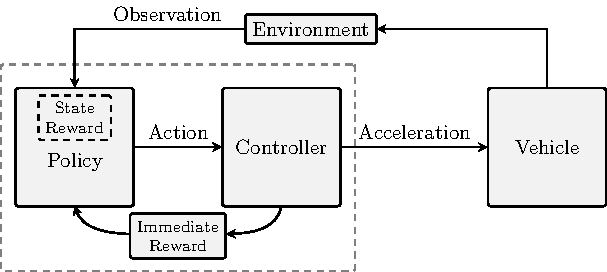
\includegraphics[width=0.8\columnwidth]{figures/figures-architecture.pdf}
	\caption{Representation of the decision making architecture}
	\label{fig:Architecture}
	\vspace{-0.3cm}
\end{figure}

%In this paper, we use reinforcement learning in combination with a Model Predictive Controller (MPC). 
A simple controller holds well when intersection crossing points are far away from each other, but when there are several crossing points in close succession, a simple controller would have a hard time handling it. In this paper, we instead propose using MPC that can consider multiple vehicles at the same time and generate an optimal trajectory. In contrast to \cite{hult}, where they prove stability and recursive feasibility using an MPC approach, and assuming that agents can cooperate, we restrict ourselves to non-cooperative scenarios. 
The MPC is used to plan trajectories around other vehicles using available predictions from other vehicles, and in the worst case, use the prediction as early detection whenever a dangerous situation, e.g., a collision, may appear. 

Applying MPC directly to the problem, could lead to a growing complexity with the number of vehicles in the intersection, e.g., which vehicle do we yield for and which vehicle do we drive in front. Therefore, we propose to separate the problem into two parts: the first being a high-level decision maker, which structures the problem, and the second being a low level planner, which optimizes a trajectory given the traffic configuration. 

For the high-level decision maker RL is used to generate decisions for how the vehicle should drive through the intersection, and MPC is used as a low-level planner to optimize a safe trajectory. Compared to \cite{decentralizedMPC} where all vehicles are controlled using MPC to stay in a break-safe set based on a model of other vehicles future trajectory, this can be perceived as too conservative for a passenger. By combining RL and MPC, the decision policy will learn which action is optimal by using feedback from the MPC controller into the reward function. Since MPC uses predefined models, e.g. vehicle models and other obstacle prediction models, the performance relies on their accuracy and assumptions. To mitigate this, we use Q-learning, which is a model-free RL approach, to optimize the expected future reward based on its experience during an entire episode which is able to compensate to some extent for model errors, which is explained more in section \ref{sec:q-learning}. 

%Using Q-learning being a model-free RL approach it optimizes the expected future reward based on its experience during an entire episode, it can therefore compensate some model errors the MPC had. e.g., if the MPC predicts a collision, the policy can choose to continue with that action anyway and still avoid a collision based on previous experience. 
%Then you may ask, why not just use MPC to solve the entire problem then? There are two drawbacks by only relying on MPC, one is the computational time that may be required to compute all possible actions for a long prediction horizon, the second limitation is large deviations from the model.  By using RL, the mixed integer problem can be solved by letting an action be one MPC solution and the policy will learn which action is the optimal by incorporating the cost function of the MPC into the reward function. Because MPC is based on models, the performance relies on the accuracy of these models and assumptions, with Q-learning being a model-free RL approach it optimizes the expected future reward based on its experience during an entire episode, it can therefore compensate some model errors the MPC had. e.g., if the MPC predicts a collision, the policy can choose to continue with that action anyway and still avoid a collision based on previous experience. 
%This is where the RL algorithm can help the MPC by solving the mixed integer problem with a Neural Network the implicitly approximates which action is the optimal one so that the MPC only have to compute the prediction for one action. The second problem the RL algorithm can help the MPC is model error, by getting a large reward based on the end of an scenario, the agent can learn to compensate for model error in the MPC by always choosing an action which yield the largest expected future reward.

This paper is structured as follows. Section \ref{sec:system} introduces the system architecture of our framework. The problem formulation, along with the two-layers of the decision algorithm is presented in Section \ref{sec:problem}. Section \ref{sec:agents} present three different used agents for simulation and validation. Implementation details is presented in Section \ref{sec:implementation} and the results are shown in Section \ref{sec:results} followed by discussion in Section \ref{sec:discussion}. Finally, conclusions and future research are presented in Section \ref{sec:conclusion}.

\

\section{System}\label{sec:system}
A full decision architecture system shown in Fig. \ref{fig:Architecture}, would include a precautionary safety layer that limits which acceleration values the system can actuate in order to stay safe. Followed by a decisions making system that makes a high level decision for when to drive in order to avoid collision and be comfortable. The policy maker later send that action to a controller that actuates the action turning it into a control signal, e.g., an acceleration request. The environment state, together with the new acceleration request, is sent though a collision avoidance system that checks if the current path has a collision risk, and mitigate if needed. With such a structure, the comfort that is experienced by the passenger is fully controlled by the low-level controller and partially affected by the decision. This paper focuses on the integration between policy and actuation, by having an MPC controller directly giving feedback to the decision maker through immediate actions. This allows the policy to know how comfortably the controller can handle the action and give feedback sooner if the predicted outcome may be good or bad. 
 

\section{Problem formulation}\label{sec:problem}
The goal of the ego-vehicle is to drive along a predefined route that has one or two intersections with crossing traffic, where the intent of the other road users is unknown. Therefore, the ego-vehicle needs to assess the driving situation and drive comfortably, while avoiding collisions with any vehicle\footnote{Although our approach can be extended to other road users, for convenience of exposition we'll refer to vehicles.} that may cross. In this section, we define the underlying Partially Observable Markov Decision Process~(POMDP) and present how the problem is decomposed using RL for decision making and MPC for planning and control.


%The objective is to drive along a main road that has one
%or two intersections with crossing traffic and control the
%acceleration in a way that avoids collisions in a comfortable
%way. All vehicles are assumed to drive along predefined
%paths on the road where they can either speed up or slow
%down to avoid collisions in the crossings. In this section the
%system architecture is defined along with the environment,
%observations and actions.

\subsection{Partially Observable Markov Decision Process}\label{sec:pomdp}
The decision making process is modeled as a Partially Observable Markov Decision Process (POMDP). A POMDP is defined by the 7-tuple $(\mathcal{S},\mathcal{A},\mathcal{T},\mathcal{R},\Omega ,\mathcal{O},\gamma)$, where $\mathcal{S}$ is the state space, $\mathcal{A}$ an action space that is defined in section \ref{sec:mpc}, $\mathcal{T}$ the transition function, %conditional transition probabilities between states
$\mathcal{R}$ the reward function $\mathcal{R}: \mathcal{S} \times \mathcal{A} \to \mathbb{R}$ is defined in \ref{sec:reward}, $\Omega$ an observation space, $\mathcal{O}$ the probability of being in state $s_{t}$ given the observation $o_t$, and $\gamma$ the discount factor.

A POMDP is a generalization of the Markov Decision Process (MDP) \cite{BellmanMDP} and therefore works in the same way in most aspects. At each time instant $t$, an action, $a_t\in \mathcal{A}$, is taken, which will change the environment state $s_t$ to a new state $s_{t+1}$. Each transition to a state $s_t$ with an action $a_t$ has a reward $r_t$ given by a reward function $\mathcal{R} $. The Key difference from a regular MDP is that the environment state $s_t$ is not entirely observable because the intention of other vehicles are not known. In order to find the optimal solution for our problem, we need to know the future intention of other drivers. Instead we can only partially perceive the state though observations $o_t\in \Omega$.

\subsection{Deep Q-Learning}
In the reinforcement learning problem, an agent observes the state $s_t$ of the environment, takes an action $a_t$, and receives a reward $r_t$ at every time step $t$. Through experience, the agent learns a policy $\pi$ in a way that maximizes the accumulated reward $\mathcal{R}$ in order to find the optimal policy $\pi^*$. In Q-learning, the policy is represented by a state action value function $Q(s_t,a_t)$. The optimal policy is given by the action that gives the highest Q-value. 
\begin{equation}
\pi^*(s_t) = \arg\max_{a_t} Q^*(s_t,a_t)
\label{eq:optimal_policy}
\end{equation}
Following the Bellman equation the optimal Q-function $Q^*(s_t,a_t)$ is given by:
 \begin{equation}
 Q^*(s_t,a_t)= \mathbb{E}[r_t + \gamma \max_{a_{t+1}} Q^*(s_{t+1}, a_{t+1})| s_t, a_t]
 \label{eq:q-function}
 \end{equation}
Because Q-learning is a model-free algorithm and it does not make any assumptions on the environment, even though models are used to simulate the environment, this can be useful when the outcome does not match the prediction models. 

\section{Agents}\label{sec:agents}
This section explains the different agents types. MPC and sliding mode (SM) for the ego vehicle. Observed target vehicles has different intention agents based on SM agent. 

\subsection{MPC agent}\label{sec:mpc}
We model the vehicle motion with states $\mathbf{x}\in\mathbb{R}^3$ and control $\mathbf{u}\in\mathbb{R}$, defined as
\begin{equation}
\mathbf{x}:=[p^\mathrm{e}\quad v^\mathrm{e}\quad a^\mathrm{e}]^\top,\quad \mathbf{u}:=j^\mathrm{e},
\end{equation}
where we denote the position along the driving path in an Frenet frame as $p^\mathrm{e}$, the velocity as $v^\mathrm{e}$, the acceleration as $a^\mathrm{e}$, and the jerk as $j^\mathrm{e}$, see Fig. \ref{fig:observations}. In addition, we assume  that measurements of other vehicles are provided through an observation  $\mathbf{o}$. We limit the scope of the problem to consider at most four vehicles, and define  the observations as
\begin{equation}
\mathbf{o} := [p^1\quad v^1\quad p^{\mathrm{cross},1}_\mathrm{ego}\quad \cdots\quad p^4\quad v^4\quad p^{\mathrm{cross},4}_\mathrm{ego}\quad ]^\top,
\end{equation}
where we denote the position along its path as $p$, the velocity as $v$, and $p^{\mathrm{cross},j}_\mathrm{ego}$ for $j\in[1,4]$, as the distance to the ego-vehicle from the intersection point, see Fig. \ref{fig:observations}.

In this paper, we assume that there exists a lateral controller that stabilizes the vehicle along the driving path. To that end, we only focus on the longitudinal control. Given the state representation, the dynamics of the vehicle is then modeled using a  triple integrator with jerk as control input.

The objective of the agent is to safely track a reference, e.g. follow a path with a target speed, acceleration, and jerk profile, while driving comfortably and satisfying constraints that arise from physical limitations and other road users, e.g. not colliding in intersections with crossing vehicles. Hence, we formulate  the  problem as a finite horizon, constrained optimal control problem
\begin{subequations}
	\label{eq:mpc}
	\begin{align}
	J = \min_{\bar\x,\bar\u} & \sum_{k=0}^{N-1}% \varphi_n(x_n,u_n) + \varphi_N(x_N)\\
	\matr{c}{\bar\x_k - \r_k^\x \\ \bar\u_k - \r_k^\u}^\top \matr{cc}{Q &S^\top\\S & R} \matr{c}{\bar\x_k - \r_k^\x \\ \bar\u_k - \r_k^\u} \\
	&\qquad + \matr{c}{\bar\x_N - \r_N^\x}^\top P \matr{c}{\bar\x_N - \r_N^\x}\nonumber\\
	&\text{s.t.}\ \ \, \bar\x_0 = \hat{\x}_0, \label{eq:mpcState}\\
	&\qquad{}\bar\x_{k+1} = A\bar\x_{k}+B\bar\u_{k},\label{eq:mpcDynamics}\\
	&\qquad{}h(\bar\x_k,\bar\u_k,\bar{\mathbf{o}}_k,a_k) \leq{} 0, \label{eq:mpcInequality}
	\end{align}
\end{subequations}
where $k$ is  the prediction time index, $N$ is the prediction horizon, $Q$, $R$, and $S$ are the stage costs, $P$ is the terminal cost, $\bar\x_k$ and $ \bar\u_k$ are the predicted state and control inputs, $\r^\x_k$ and $\r^\u_k$ are the state and control input references, $\bar{\mathbf{o}}_k$ denotes the predicted state of vehicles in the environment which need to be avoided, and $a$ is the action from the high-level decision maker. Constraint \eqref{eq:mpcState} enforces that the prediction starts  at the current state estimate $\hat\x_0$, \eqref{eq:mpcDynamics} enforces the system dynamics, and \eqref{eq:mpcInequality} enforces constraints on the states, control inputs, and obstacle avoidance.

The reference points, $\r^\x_k$, $\r^\u_k$ are assumed to be set-points of a constant velocity trajectory, e.g. following the legal speed-limit on the road. Therefore, we set the velocity reference according to the driving limit, and the acceleration and jerk to zero.

\subsubsection{Obstacle prediction}
In order for the vehicle planner in \eqref{eq:mpc} to be able to properly avoid collisions, it is necessary to provide information about the surrounding vehicles in the environment. Therefore, similarly to \cite{batkovic2019}, we assume that a sensor system provides information about the environment, and that there exists a prediction layer which generates future motions of other vehicles in the environment. The accuracy of the prediction layer will heavily affect the performance of the planner, hence, it is necessary to have computationally inexpensive and accurate prediction methods.

In this paper, for simplicity the future motion of other agents is estimated by a constant velocity prediction model. The motion is predicted at every time instant for prediction times $k\in[0,N]$, and is used to form the collision avoidance constraints, which we describe in the next section. Even though more accurate prediction methods do exist, e.g. \cite{lefevre2014survey,batkovic2018}, we use this simple model to show the potential of the overall framework.

\subsubsection{Collision avoidance}
\begin{figure}[t]
	\centering
	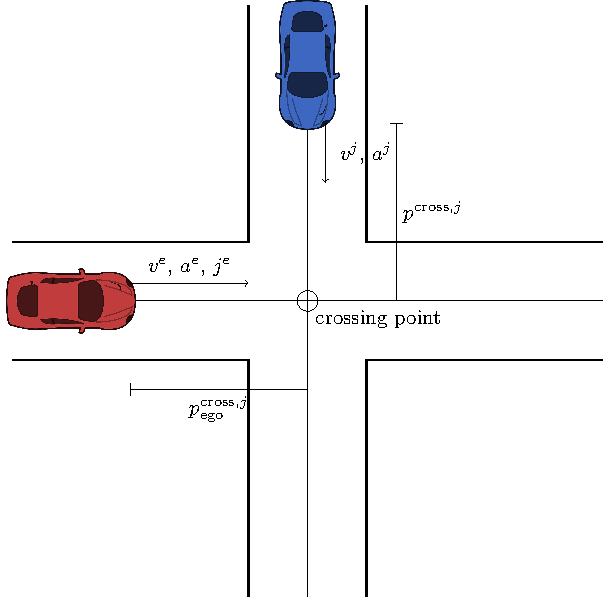
\includegraphics[width=0.6\columnwidth]{figures/figures-observations.pdf}
	\caption{Observations of a scenario}
	\label{fig:observations}
\end{figure}\
We denote a vehicle $j$ with the following notation $\x^j:=[p^j\, v^j\, a^j]^\top$, and an associated crossing point at position $p^{\mathrm{cross},j}$ in its own vehicle frame, which translated into the ego-vehicle frame is denoted as $p^{\mathrm{cross},j}_\mathrm{ego}$. With a predefined road topology, we assume that the vehicles will travel along the assigned paths, and that collisions may only occur at the crossing points $p^{\mathrm{cross},j}$ between an obstacle and the ego vehicle. Hence, for collision avoidance, we use the predictions of the future obstacle states $\bar\x^j_k$ for times $k\in[0,N]$, provided by a prediction layer outside of the MPC framework. Given the obstacle measurements, the prediction layer will generate future states throughout the prediction horizon. With this information, it is possible to identify the time slots when an obstacle will enter the intersection.

Whenever an obstacle $j$ is predicted to be within a threshold of $p^{\mathrm{cross},j}$, e.g. the width of the intersecting area, the ego vehicle faces a constraint of the following form
\begin{gather*}
\bar{p}_k^\mathrm{e} \geq{} p^{\mathrm{cross},j}_\mathrm{ego} + \Delta,\quad\underline{p}_k^\mathrm{e} \leq{} p^{\mathrm{cross},j}_\mathrm{ego} - \Delta,
\end{gather*}
where $\Delta$ ensures sufficient padding from the crossing point that does not cause a collision. The choice of $\Delta$ must be at least such that $p_k$ together with the dimensions of the ego-vehicle does not overlap with the intersecting area.

\subsubsection{Take way and give way constraint}
Since the constraints from the surrounding obstacles become non-convex, we rely on the high-level policy maker to decide through action $a$ how to construct the constraint \eqref{eq:mpcInequality} for Problem \eqref{eq:mpc}. The take-way action implies that the ego-vehicle drives first through the intersection, i.e., it needs to pass the intersection before all other obstacles. This implies that for any vehicle $j$ that reaches the intersection during prediction times $k\in[0,N]$, the generated constraint needs to lower bound the state $p_k$ according to
\begin{equation}
\max_{j}p^{\mathrm{cross},j}+\Delta \leq{}p_k^\mathrm{e}.
\end{equation}
Similarly, if the action is to give way, then the position needs to be upper bounded by the closest intersection point so that
\begin{equation}
p_k^\mathrm{e} \leq{} \min_{j}p^{\mathrm{cross},j}_\mathrm{ego}-\Delta,
\end{equation} 
for all times $k$ that the obstacle is predicted to be in the intersection.

\subsubsection{Following an obstacle}
For any action $a$ that results in the following of an obstacle $j$, the ego-vehicle position is upper bounded by $p^\mathrm{e}_k \leq{} p^\mathrm{cross,j}_\mathrm{ego}$. We construct constraints for obstacles $i\neq{}j$ according to
\begin{itemize}
	\item if $p^\mathrm{cross,i}<{}p^\mathrm{cross,j}$ then $p^\mathrm{cross,i}+\Delta\leq{}p_k^\mathrm{e}$, which implies that the ego-vehicle should drive ahead of all obstacles $i$ that are approaching the intersection;
	\item if $p^\mathrm{cross,i}>{}p^\mathrm{cross,j}$ then $p_k^\mathrm{e}\leq{}p^\mathrm{cross,i}-\Delta$, which implies that the ego-vehicle should wait to pass obstacle $j$ and other obstacles $i$;
	\item if $p^{\mathrm{cross,i}}=p^{\mathrm{cross},j}$ then the constraints generated for obstacle $i$ becomes an upper or lower  bound depending on if obstacle $i$ is ahead or behind the obstacle $j$ into the intersection.
\end{itemize}

\subsection{Sliding mode agent}
To benchmark the performance of using MPC, a SM controller that was used in \cite{Tram2018} is introduced. 
\begin{subequations}
	\label{eq:sliding_mode}
	\begin{align}
	a^e_{sm} &= \frac{1}{c_2} (- c_1 x_2 + \mu sign(\sigma(x_1, x_2))), \\
	&\text{where}
	\begin{cases}
	x_1 = p^t - p^e,\\
	x_2 = v^t - v^e,
	\end{cases}\\
	&\sigma = c_1 x_1 + c_2 x_2,\\
	\label{eq:p-controller}
	&a^e_\mathrm{p} = K (v_{\mathrm{max}} - v^e),\\
	\label{eq:final_acc}
	&a^e = \min(a^e_{\mathrm{sm}}, a^e_\mathrm{p} ).
	\end{align}
\end{subequations}
The SM controller aims to keep a minimum distance to a target car with a velocity of $v^e$, by controlling the acceleration $a^e_{\mathrm{sm}}$. $c_1$, $c_2$, and  $\mu$ are tuning parameters to control the comfort of the controller. In case there is no target car, the controller maintains a target velocity $v_{\mathrm{max}}$ with a regular p-controller from \eqref{eq:p-controller} with a proportional constant $K$. The final acceleration is given by \eqref{eq:final_acc}. For more details about the SM agent see \cite{Tram2018}.

\begin{figure}[t!]
	\centering
	\vspace{0.3cm}
	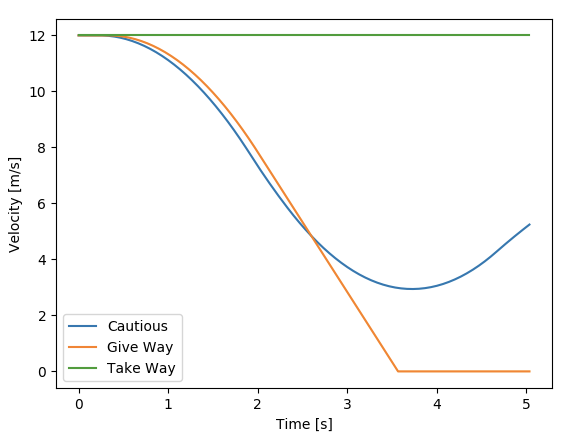
\includegraphics[width=0.7\columnwidth]{figures/velocity_profiles_agents.png}
	\caption{Example of how velocity profile of the different intention agents can look like. All agents has the same starting velocity of $12$m/s and are approaching the same intersection}
	\label{fig:intention_profiles}
	\vspace{-0.3cm}
\end{figure}\
\subsection{Intention agents}

There are three different intention agents for crossing traffic with predetermined intentions, three velocity profiles are shown as an example in Fig. \ref{fig:intention_profiles}. All agents were implemented with a SM controller with different target values. The take way intention does not yield for the crossing traffic and simply aim to keep its target reference speed. Give way intention however, slow down to a complete stop at the start of the intersection until crossing traffic has passed before continuing through. The third intention is cautious, slowing down but not to a full stop. This makes it difficult for a constant velocity or acceleration model to predict what other agents will do.
\section{Implementation}\label{sec:implementation}

\subsection{Deep Q-Network}
\begin{figure}[t]
	\centering
	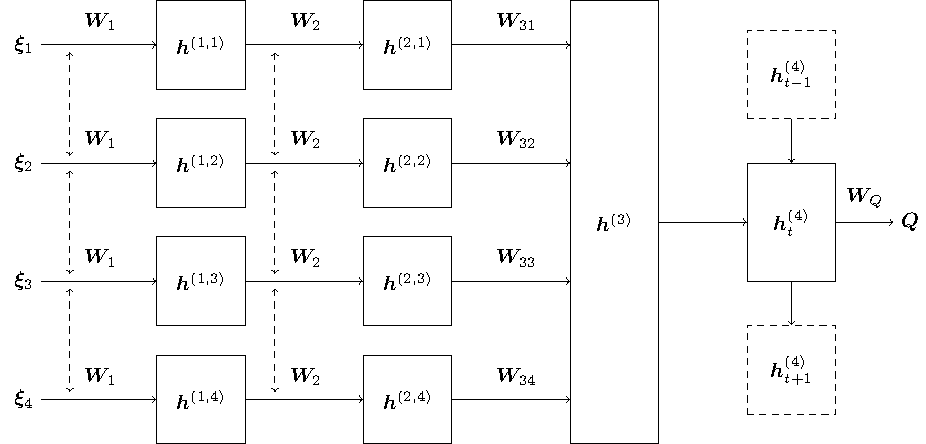
\includegraphics[width=0.95\columnwidth]{figures/figures-network.pdf}
	\caption{Representation of the network structure}
	\label{fig:Network}
\end{figure}
\label{sec:q-learning}
The deep Q-network is structured as a three layer neural network with shared weights and a Long Short-Term Memory based on previous work \cite{Tram2018} and shown in Fig. \ref{fig:Network}. The input features $\xi_n$ are composed of observations $o_t$, introduced in section \ref{sec:pomdp} and shown in Fig. \ref{fig:observations}, with up to four observed vehicles: 
%, our findings showed the importance of sharing the weights for different target vehicles, similar work by Hoel et al. \cite{Hoel} but with a Convolutional Nerual Network and a pooling layer also come to the same conclusion. 

%\vspace{0.3cm}
\begin{equation}
	\begin{aligned}
	&\xi_1 = [\  p^e_t \quad v^e_t \quad a^e_t \quad \delta^e \quad p^1_t \quad v^1_t \quad a^1_t \quad \delta^1 \  ]^T\\
	&\xi_2 = [\  p^e_t \quad v^e_t \quad a^e_t \quad \delta^e \quad p^2_t \quad v^2_t \quad a^2_t \quad \delta^2 \  ]^T\\
	&\xi_3 = [\  p^e_t \quad v^e_t \quad a^e_t \quad \delta^e \quad p^3_t \quad v^3_t \quad a^3_t \quad \delta^3 \  ]^T\\
	&\xi_4 = [\  p^e_t \quad v^e_t \quad a^e_t \quad \delta^e \quad p^4_t \quad v^4_t \quad a^4_t \quad \delta^4 \  ]^T\\
	\end{aligned}
\end{equation}
%\vspace{0.3cm}

Normalization of the input features is done by scaling the features down to values between $[-1,1]$ using the maximum speed $v_{\max}$, maximum acceleration $a_{\max}$ and a car's sight range $p_{\max}$. Empty observation of other vehicles $[p^n_t \quad v^n_t \quad a^n_t \quad \delta^n ]$ has a default value of $-\mathbf{1}$. The input vectors are sent though two hidden layers $\bm{h}^{(1, i)}$ and $\bm{h}^{(2, i)}$ with shared weights $\bm{W}_1$ and $\bm{W}_2$ respectively
\begin{equation}
\bm{h}^{(1, i)} = \tanh\left(\bm{W}_1 \bm\xi_i + \bm{b}_1\right)
\end{equation}
\begin{equation}
\bm{h}^{(2, i)} = \tanh\left(\bm{W}_2 \bm{h}^{(1, i)} + \bm{b}_2\right).
\end{equation}
A similar study for lane changes on a highway confirmed the importance of having equals weights for inputs that describe the state of interchangeable objects \cite{Hoel}. The output of each sub-network is then sent though a fully connecting layer 
%The output of each sub-network, $\bm{h}^{(2, i)}$ and $\bm h^{(ego)}$,  is fed as input into a third hidden layer $\bm{h}^{(3)}$.
%The different sub-networks' $\bm{h}^{(2, i)}$ outputs are multiplied with different weights $\bm{W}_{31},\dots,\bm{W}_{34}$ in order to distinguish different cars for different follow car actions. The ego features are also fed into layer 3 with its own weights $\bm{W}^{(ego)}_2$. The neurons in layer $\bm{h}^{(3)}$ combine the inputs by adding them together:
\begin{equation}
\label{eq:shared_weights}
\bm{h}^{(3)} = \tanh\left(\sum_{i=1}^4 \bm{W}_{3i} \, \bm{h}^{(2, i)} + \bm{b}_3\right).
\end{equation}
That is then connected to an Long Short-Term Memory (LSTM) \cite{Hochreiter1997LONGMEMORY} that can store and use previous features
%The final layer $\bm{h}^{(4)}$ uses the LSTM, described in section \ref{sec:method}. This layer handles the storage and usage of previous observations, making it the recurrent layer of the network. 
\begin{equation}
\bm{h}^{(4)}_t = \text{LSTM}\left( \bm{h}^{(3)} | \bm{h}^{(4)}_{t-1} \right).
\end{equation}
The approximated Q-value is then
\begin{equation}
\bm{Q}_{approx} = \bm{W}_Q \bm{h}^{(4)}+ \bm{b}_4
\end{equation}
The Q-value is then masked using Q-masking, explain in section \ref{sec:masking}
\begin{equation}
\bm{Q} = \bm{Q}_{approx}  \bm{Q}_{mask}
\end{equation}
the optimal policy $\pi^*$ is then given by taking the action that gives the highest Q-value
\begin{equation}
\pi^*(s_t) = \arg\max_{a_t} Q^*(s_t,a_t)
\end{equation}

\subsection{Q-masking}
\label{sec:masking}
Q-masking \cite{Mukadam2017} helps the learning process by reducing the actions space by disabling actions the agent does not need to explore. If there are less than $N$ cars, it would then be meaningless to choose to follow a car that does not exist. Which motivates masking off cars that does not exist. In previous work \cite{Tram2018}, a high negative reward was given when an action to follow a car that did not exist was chosen, while the algorithm continued with a default action take way. The agent quickly learned to not choose cars that did not exist, but with Q-masking, the agent does not even have to explore these options. For other details about the training see \cite{Tram2018}.

\subsection{Simulation environment}
All agents are spawned with random initial speed $v_0 \in [10,30]$m/s, position $p^i_0 \in [10,55]$m and intention. The cars dimensions are $2$ m wide and $4$ m long. The ego car operates within comfort bounds and therefore has a limited maximum acceleration and deceleration of $5$ m/s$^2$. 
\begin{figure}[t]
	\centering
	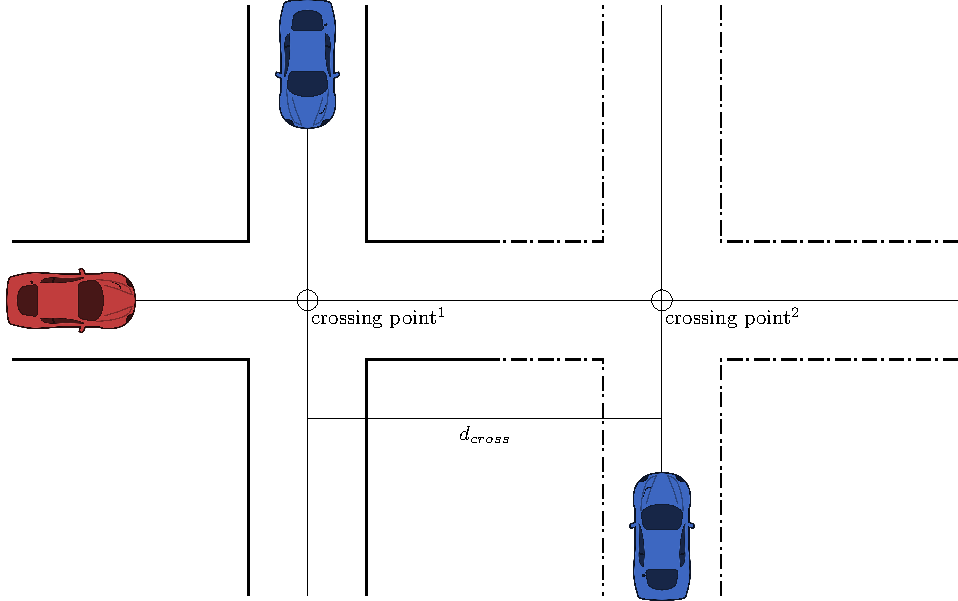
\includegraphics[width=.95\columnwidth]{figures/figures-scenarios.pdf}
	\caption{Illustration of a intersection scenario, where the solid line is a single crossing and together with the dashed line creates a double crossing.}
	\label{fig:scenario}
\end{figure}
Two main types of crossing were investigated. One and two crossing points as shown in Fig. \ref{fig:scenario}, where the distance between crossing points $d_{cross}$ vary between $[4, 8, 12, 25, 30, 40] m$ with different scenarios. 

The MPC agent was discretized at $30$Hz, with a prediction horizon of $N=100$ and cost tuning of
\begin{gather}
Q=\mathrm{blockdiag}(0.0,1.0,1.0),\ R=1,\ S=\mathbf{0}.
\end{gather}

\subsection{Reward function tuning}\label{sec:reward}
There are three states that terminates an episode; success, failure, and timeout. Success is when the ego agent reaches the of the road defined by the scenario. Failure is when the frame of the ego agent overlaps with another road users frame, e.g., in a collision, this frame can be the size of the vehicle or a safety boundary around a vehicle. The final terminating state is timeout and that is simply when the agent cant reach the two previous terminating states before the timeout time $ \tau_m$.
According to \cite{VanHasseltLearningMagnitude}, the $Q_\pi$ values and gradient can grow to be very large if the total reward values are too large. All rewards are therefore scaled with the episode timeout time $\tau_m$, which is set to 25$s$, to keep the total reward $r_t \in [-2, 1]$.
The reward function is defined as follows:
\begin{align*}
r_t = &\begin{cases}
1 & \text{on success, }\\
-1                & \text{on failure},\\
0.5                 & \text{on timeout, i.e. } \tau \ge \tau_m,\\
% \text{mpc cost function}   & \text{on non-terminating updates} \in [-1, 0]\\
f(p_{\text{crash}}, p_{\text{comf}}) & \text{on non-terminating updates},\\
% -\left(\frac{j^{e}_t}{j_{\max}}\right)^2\frac{\Delta \tau}{\tau_m}         & \text{on non-terminating updates}
\end{cases} 
\end{align*}
where $f(p_{\text{crash}}, p_{\text{comf}})$ consists of
\begin{equation}
f(p_{\text{crash}}, p_{\text{comf}})  = \alpha p_{\text{crash}}  \frac{\tau_m}{\tau - t_{pred}} + \beta p_{\text{comf}} \frac{\tau_m}{\tau},
\label{eq:mpc_reward}
\end{equation}
with  $\alpha\in[0,1]$, $\beta\in[0,1]$ being weight parameters, and $\alpha+\beta=1$. The first term in the function corresponds to a feasibility check of Problem \eqref{eq:mpc}, which to a large extent depends on the validity of the accuracy of the prediction layer. The high-level decision from the policy-maker affects how the constraints are constructed, and may turn the control problem infeasible, e.g. if the decided action is to take way, while not being able to pass the intersection before all other obstacles. Therefore, whenever the MPC problem becomes infeasible we set $p_\mathrm{crash}=1$ to indicate that the selected action most likely will result in a collision with the surrounding environment.

The second term $p_\mathrm{comf}$ relates to the comfort of the planned trajectory, which is estimated by computing and weighting the acceleration and jerk profiles as
\begin{align*}
p_\mathrm{comf} = \frac{1}{\sigma{}N}(\sum_{k=0}^{N-1} \bar{a}_k^2Q^a + \bar{j}_k^2R^j + a_N^2Q^a),
\end{align*}
where $\bar{a}$, and $\bar{j}$ are the acceleration and jerk components of the state and control input respectively, $Q^a$ and $R^j$ are the corresponding weights, and $\sigma$ is a normalizing factor which ensures that $p_\mathrm{comf}\in[0,1]$. For the simulation we used $Q^a=1$ and  $R^j=1$.

The timeout reward 0.5 was set to be higher than the average accumulated reward from $p_\mathrm{comf}$, so that the total accumulated reward would be positive in case of timeouts. Because $p_{\text{crash}}$ usually only triggers close to a potential collision, that is why $t_{pred}$ is set to the first time a crash prediction is triggered. This will scale the negative reward higher in collision episodes. 

\section{Results}\label{sec:results}
For evaluation we compared the success rate of the decision-policy together with a collision to timeout ratio~(CTR). The success rate is defined as the number of times the agent is able cross the intersections without colliding with other obstacles, or exceeding the time limit to cross. Since we define a time-out to be a failure, we use the CTR to separate potential collisions with the agent being too conservative.

Fig. \ref{fig:result1} shows a comparison in success rate between the proposed MPC architecture and the previous SM agent for scenarios with only one crossing. In this scenario, the MPC agent converges after $10^4$ training episodes, while the previous SM agent converges after $4\cdot{}10^4$ training episodes. In addition, comparing the CTR metric, Fig. \ref{fig:result2} shows that the MPC agent has $0.45$ CTR while the SM agent has $0.72$ CTR. Evidently, it is visible that the MPC is able to leverage future information into its planning horizon in order to achieve faster training, and also avoiding collisions as a  result.

We evaluate the performance of the MPC and SM agents for the more difficult double intersection problem, where we vary the distance between the intersection points. Table \ref{tab:successrate} shows the performance of the MPC and SM agent for both the single and double scenarios. The performance drops for both agents for the double crossing scenario. However, it is visible that the MPC agent suffers less performance degradation compared to the SM agent. The CTR however more than doubles for the MPC agent for the double crossing, while the already high CTR rate for the SM agent increases above rates of $0.9$.

\begin{figure}[t!]
	\centering
	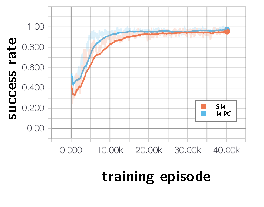
\includegraphics[width=\columnwidth]{figures/figures-successrate.pdf}
	\vspace{-3.5em}
	\caption{Average MPC and SM success rate for a single corssing after evaluating the policy 300 episodes.}
	\label{fig:result1}
\end{figure}

\begin{figure}[t!]
	\centering
	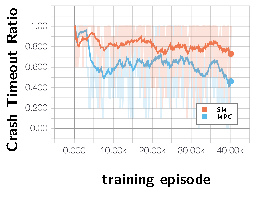
\includegraphics[width=\columnwidth]{figures/figures-crashratio.pdf}
	\vspace{-4em}
	\caption{Average MPC and SM crash to timeout ratio for a single crossing after evaluating the policy in 300 episodes. A CTR of $0$ means that all failures are timeouts, while a CTR of $1$ means that all failures are collisions.}
	\label{fig:result2}
\end{figure}

\begin{table}[t!]
	\centering
	\caption{Average success rates and collision to timeout rates.}% across single and double crossings.}   
\begin{tabular}{ |p{1,6cm}||p{1,2cm}|p{1,2cm}|p{1,2cm}|p{1,2cm}|}
	% \begin{tabular}{ |p{1,3cm}||p{0,8cm}|p{0,8cm}|p{0,8cm}|p{0,8cm}|}
	\hline
	Controller &\multicolumn{2}{|c|}{Success Rate}
	&\multicolumn{2}{|c|}{Timeout Ratio}\\
	\hline
	 & Single & Double & Single & Double\\
	\hline
	SM & $96.1\%$ & $90.9\%$ & $72\%$ & $93\%$\\
	MPC & $97.3\%$ & $95.2\%$ & $45\%$ & $76\%$\\
	\hline
\end{tabular}
\label{tab:successrate}
\end{table}
\section{Discussion}\label{sec:discussion}
The benefit of being able to use a prediction horizon for the MPC is shown to mostly impact the training time for the traffic scenarios compared to the SM agent. This allows the RL decision-policy to get feedback early in the training process to see whether an action most likely will lead to a collisions. In addition, the lower CTR also implies that the use of a prediction horizon also makes the decision-policy more conservative, since it rather times out than risk collisions.

It is important to note little effort was put into tuning the MPC agent, and that we used very primitive prediction methods that do not hold very well in crossing scenarios, e.g. the simulated agents did not keep constant speed profiles while approaching the intersections. However, under these circumstances, the decision algorithm still managed  to obtain a success rate above  $95\%$ for the double crossings.

%It is also important to note that the MPC was not optimally tuned and very simple models were used in this experiments. Nevertheless the policy could compensate for the model errors and still find a policy that succeed $97\%$ of the time. 
\section{Conclusion}\label{sec:conclusion}
In this paper, we proposed a decision making algorithm for intersections which consists of two components: a high-level decision maker that uses Deep Q-learning to generate decisions for how the vehicle should drive through the intersection, and a low-level planner that uses MPC  to optimize safe trajectories. We tested the framework in a traffic simulation with randomized intent of other road users for both single and double crossings. Results showed that the proposed MPC agent outperforms the previous SM agent by almost $5\%$ in scenarios with double crossings and in cases of failure, more often timeout than colliding.
